\section{Introduction}
3D printing enables the fabrication of complex geometry under few design constraints compared to conventional fabrication techniques.
Recent developments have seen a rapid growth in both the use and capabilities of desktop 3D printing systems.
%The rapid spread of 3D printing through different industries and types of application calls for the possibility to manufacture a wide range of geometries while guaranteeing mechanical properties of the resulting parts.
Fused Deposition Modeling (FDM) is one of the most common 3D printing techniques.
It is widely used because of the versatility in the types of plastic which can be used and the relatively low running costs.
FDM printers are used, for example, in showcasing scale models of buildings, casings for electronics, prototypes for blow molded parts, jigs and fixtures.
Recent research \revise{developments have investigated}{adressed} manufacturing complex volumetric structures such as microstructures~\cite{bates2018compressive,Al-Ketan2018,Maskery2018} and topology optimized structures~\cite{Zegard2016SMO,Wu2019a,Cheng2019}.
Many of these applications involve 3D models with detailed features within the order of magnitude of the \revise{printing resolution}{nozzle size}, which restrains the field of the process planning algorithms.

FDM printers extrude semi-continuous beads of molten plastic through a nozzle, which moves along a planned toolpath within each layer of a 3D object.
\revise{
A common strategy to accurately manufacture a given 3D model is to extrude along a contour-following path,
because the position and shape of the toolpath can be controlled relatively accurately.
Filling up a shape using parallel straight lines would expose defects of the size of the hole in the nozzle, which is generally an order of magnitude larger than the resolution of the positioning system.
Contour-parallel extrusion therefore leads to a less bumpy outline shape than direction-parallel extrusion does.
}{%sgd
A common strategy is to extrude along a number of parallel toolpaths which follow the shape of the contour of the layer and fill up the remaining area using parallel straight toolpaths.
Contour-parallel toolpaths fit to the layer outlines more accurately, because the resolution of the positioning system is an order of magnitude smaller than the size of the hole in the nozzle.
This paper is concerned with the generation of such contour-parallel toolpaths and addresses several issues which commonly occur in 3D models with narrow geometry.
%Because contour-parallel extrusion leads to a more accurate outline shape it is common practice to print either the whole layer or only a limited number of outer perimeters that way.
%This paper improves on those contour-parallel toolpaths and addresses several issues which commonly occur in 3D models with narrow geometry.
}


The simple technique for generating the dense contour-parallel toolpaths of a layer consists \revise{in}{of} performing uniform inward offsets with the size of the nozzle from the outline shape.
However, for geometrical features which are not an exact multiple of the nozzle size this method produces areas where an extrusion bead is placed twice: \emph{overfill} areas; and areas which are not filled at all: \emph{underfill} areas.
See \cref{intro_wedge_uniform}.
Overfills cause a buildup of pressure in the mechanical extrusion system, which can result in bulges or even a full print failure.
Underfills\revise{}{,} on the other hand, can cause a drastic decrease in the part stiffness or even for small features not to be printed at all.
These problems are exacerbated for models with layer outlines with small features, because the over- and underfill areas are relatively large compared to the \revise{whole part}{those features}.

One promising direction to avoid over- and underfills is to employ toolpath\revise{}{s} with adaptive width.
\citeauthor{Ding2016a} developed a toolpath strategy for wire and arc additive manufacturing which produces a width variation typically lower than a factor of $3$, but is \revise{sometimes}{} far greater\revise{}{ for some parts}~\cite{Ding2016a,Xiong2019}.
However, the range of \revise{}{bead }widths manufacturable by FDM systems is limited.
A nozzle of \revise{\SI{0.4}{\milli\meter}}{$w=\SI{0.4}{\milli\meter}$} will typically start to cause fluttered extrusion around lines narrower than \SI{0.3}{\milli\meter} and lines will start to bulge upward if they are wider than the flat part of the nozzle, which is typically \SI{1.0}{\milli\meter}.
%Therefore, a limited range of widths is required by the hardware system.

The current \revise{state-of-the-art}{state of the art of contour-parallel toolpath generation} \revise{for FDM printing }{}developed by \citeauthor{Jin2017JMS}
employs a strategy which alters the widths of the centermost beads \revise{at most by a factor of $2$}{within a range of widths $[0.25w,1.8w]$}~\cite{Jin2017JMS},
which is similar to the strategy employed by the open source industry standard software package Ultimaker Cura~\cite{cura}.
See \cref{intro_wedge_centered}.
Still, controlling the extrusion width through movement speed changes or through volumetric flow control (e.g. linear advance) yields diminishing accuracy for deposition widths \revise{farther away}{deviating more} from the nozzle size,
since process parameters such as nozzle temperature are optimized for beads with the nozzle size.
Moreover, reducing the variation in width is beneficial for limiting the variation in mechanical properties of the resulting product, meaning it conforms better to a simulation which employs a homogeneity assumption.
\revise{
Therefore, a narrower range of widths is desirable.
}
{We therefore reduce the bead width range by distributing the workload from the centermost bead over neighboring beads.}

\revise{
In this paper we propose a framework for planning toolpaths with control over the adaptive width for minimizing over- and underfill
We show that this framework supports various control schemes for determining the bead spacing and extrusion widths. 
For FDM printing in particular we propose a novel scheme which reduces the amount of over- and underfill while ensuring the extrusion beads deviate little from the nozzle size.
See \cref{intro_wedge_distributed}. 
}{}

\begin{figure}\centering
\setlength{\figwidth}{.9\columnwidth}
\setlength{\figwidthTwo}{.05\columnwidth}
\begin{subfigure}{\figwidth}\centering
\parbox[b]{\figwidthTwo}{\subcaption{}\label{intro_wedge_uniform}}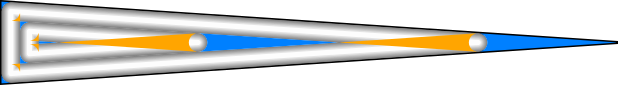
\includegraphics[width=\figwidth]{sources-intro-TEST-naive-accuracy.png}
\end{subfigure}
\begin{subfigure}{\figwidth}\centering
\parbox[b]{\figwidthTwo}{\subcaption{}\label{intro_wedge_centered}}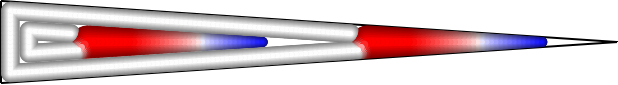
\includegraphics[width=\figwidth]{sources-intro-TEST-Center-widths.png}
\end{subfigure}
\begin{subfigure}{\figwidth}\centering
\parbox[b]{\figwidthTwo}{\subcaption{}\label{intro_wedge_distributed}}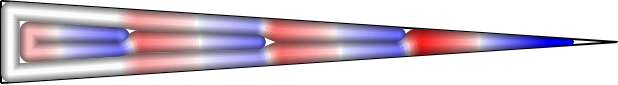
\includegraphics[width=\figwidth]{sources-intro-TEST-Distributed-widths.png}
\end{subfigure}
\caption{
Illustration of different toolpath\revise{}{s} for a \revise{wedge }{}shape \revise{}{showcasing a range of shape radii }\revise{}{(black)}.
\revise{}{These results can be read as a graph with feature size on the horizontal axis and its corresponding beading along the vertical axis.}
\subref{intro_wedge_uniform} Toolpath\revise{}{s} using uniform offsetting results in large overfill (orange) and underfill (azure).
\subref{intro_wedge_centered} Toolpath\revise{}{s} with adaptive width~\cite{Jin2017JMS} where beads that are wider or narrower than the nozzle size are \revise{indicatd}{indicated} in red and blue, respectively.
\subref{intro_wedge_distributed} Our approach minimizes over- and underfill with \revise{beads close to the nozzle size}{less extreme widths}.
}
\label{intro_wedge}
\end{figure}


Our contributions are as follows:
\begin{itemize}
\item A geometric framework \revise{for generating densely filling contour-parallel toolpaths employing adaptive width, according to any beading scheme which decides on the bead spacing and widths.}{allowing various adaptive bead width control schemes used to generate contour-parallel toolpaths which minimize under- and overfill.}
\item A specific beading scheme\revise{ for FDM printing}{,} which
reduces the \revise{amount of deviation}{variation} in the extrusion widths \revise{compared to existing literature, }{to within $[0.75w,1.5w]$.}
\revise{and which promotes smooth toolpaths that are equal to the preferred width toward the outline of the shape.}{}
\revise{}{
\item A back pressure compensation approach to accurately realize adaptive bead width on Bowden style hardware systems.
}
\end{itemize}

%This work is patent pending, but the source code is available open source.

